% Standard stuff
	\documentclass[a4paper,10pt,norsk]{article}
	\usepackage[utf8]{inputenc}
	\usepackage[norsk]{babel}
	\usepackage{amsmath,graphicx,varioref,verbatim,amsfonts,geometry,enumerate,commath,tcolorbox}
	% colors in text
	\usepackage[usenames,dvipsnames,svgnames,table, colorlinks]{xcolor, hyperref}
	% Hyper refs
	%inkspace
	\usepackage{import}
	\usepackage{xifthen}
	\usepackage{pdfpages}
	\usepackage{transparent}

%Colour scheme for hyperlinks
	\hypersetup{%
		colorlinks,
		citecolor=blue,
		linkcolor=blue,
		urlcolor=blue}

% Document formatting
	\setlength{\parindent}{0mm}
	\setlength{\parskip}{1.5mm}

%Color scheme for listings
	\usepackage{textcomp}
	\definecolor{listinggray}{gray}{0.9}
	\definecolor{lbcolor}{rgb}{0.9,0.9,0.9}

%Listings configuration
	\usepackage{listings}
	\lstset{%
		backgroundcolor=\color{lbcolor},
		tabsize=4,
		rulecolor=,
		language=python,
		basicstyle=\scriptsize,
		upquote=true,
		aboveskip={1.5\baselineskip},
		columns=fixed,
		numbers=left,
		showstringspaces=false,
		extendedchars=true,
		breaklines=true,
		prebreak = \raisebox{0ex}[0ex][0ex]{\ensuremath{\hookleftarrow}},
		frame=single,
		showtabs=false,
		showspaces=false,
		showstringspaces=false,
		identifierstyle=\ttfamily,
		keywordstyle=\color[rgb]{0,0,1},
		commentstyle=\color[rgb]{0.133,0.545,0.133},
		stringstyle=\color[rgb]{0.627,0.126,0.941}
	}

%new commands
	\renewcommand{\lstlistingname}{Kode}
	\renewcommand{\lstlistlistingname}{\lstlistingname}
	\newcommand{\dd}[1]{\mathrm{d}#1}
	\def\doubleunderline#1{\underline{\underline{#1}}}

	\newcommand{\incfig}[2][1]{%
		\def\svgwidth{#1\columnwidth}
		\import{./figures/}{#2.pdf_tex}
	}
	\pdfsuppresswarningpagegroup=1
%opening
	\title{}
	\author{%
		Christophe Blomsen\\
		\texttt{\href{mailto:chriskbl@student.matnat.uio.no}{chriskbl@student.matnat.uio.no}}
		}

\begin{document}
%Titlepage
	\begin{titlepage}
	\maketitle
	\tableofcontents
	\listoffigures
	\lstlistoflistings

	\end{titlepage}

%oppgave a
	\addcontentsline{toc}{section}{a)}
	\section*{a)}\label{ass:a}
	All kode vil ligge i samme python fil så de relevante kode snuttene er tilgjengelig på de tilsvarende deloppgavene. Hele filen kan finnes i Appendikset.
	\begin{lstlisting}[caption=Kode oppgave a)]
import scipy.io as sio
import numpy as np
import matplotlib.pyplot as plt

data = sio.loadmat('data.mat')
x = data.get('x')
y = data.get('y')
u = data.get('u')
v = data.get('v')
xit = data.get('xit')
yit = data.get('yit')

print(np.shape(x))
print(np.shape(y))
print(np.shape(u))
print(np.shape(v))
print(np.shape(xit))
print(np.shape(yit))

print(x)
print(y)
	\end{lstlisting}
	Utskrift til terminalen blir
	\begin{tcolorbox}
		x shape is (201, 194)\\
		y shape is (201, 194)\\
		u shape is (201, 194)\\
		v shape is (201, 194)\\
		xit shape is (1, 194)\\
		yit shape is (1, 194)\\
		\text{[[ 0. 0.5  1.  ... 95.5 96.  96.5]}\\
		\text{[ 0.   0.5  1.  ... 95.5 96.  96.5]}\\
		\text{[ 0.   0.5  1.  ... 95.5 96.  96.5]}\\
		...\\
		\text{[ 0.   0.5  1.  ... 95.5 96.  96.5]}\\
		\text{[ 0.   0.5  1.  ... 95.5 96.  96.5]}\\
		\text{[ 0.   0.5  1.  ... 95.5 96.  96.5]]}\\
		\text{[[-50.  -50.  -50.  ... -50.  -50.  -50. ]}\\
		\text{[-49.5 -49.5 -49.5 ... -49.5 -49.5 -49.5]}\\
		\text{[-49.  -49.  -49.  ... -49.  -49.  -49. ]}\\
		...\\
		\text{[ 49.   49.   49.  ...  49.   49.   49. ]}\\
		\text{[ 49.5  49.5  49.5 ...  49.5  49.5  49.5]}\\
		\text{[ 50.   50.   50.  ...  50.   50.   50. ]]}\\
	\end{tcolorbox}
	Ser da at griddet i $xy$-planet har et regulært intervall på $0.5$ mm i begge rettninger. Samt at $y$-koordinatene spenner ut hele diameteren til røret.
%oppgave b
	\addcontentsline{toc}{section}{b)}
	\section*{b)}\label{ass:b}
	Observerer fra presentasjonen av eksperimentet at det er væskefase i den nedre halvdelen av røret og gassfase i den andre halvdelen.
	\begin{lstlisting}[caption=Kode oppgave b]
velocity = np.sqrt(u**2 + v**2)

plt.subplot(2, 1, 1)
plt.plot(xit, yit, "k*")
water_bender = plt.contourf(x, y, velocity, np.linspace(0, 500, 100))
plt.colorbar(water_bender)

plt.subplot(2, 1, 2)
plt.plot(xit, yit, "k*")
air_bender = plt.contourf(x, y, velocity, np.linspace(1000, 5000, 100))
plt.colorbar(air_bender)

plt.savefig("oppgave_b.png")
plt.show()
	\end{lstlisting}
	Det produserer følgende \hyperref[fig:b]{plot}
%oppgave c
	\addcontentsline{toc}{section}{c)}
	\section*{c)}\label{ass:c}
	Velger å bruke vært femte element i pilplottet
	\begin{lstlisting}[caption=Kode til oppgave c]
def rectangle(x1, x2, y1, y2):
    position1 = (x[x2, x1], y[x2, y1])
    position2 = (x[y2, y1], y[y2, y1])

    # Bottom
    plt.plot([position1[0], position2[0]], [position1[1], position1[1]], "r")

    # Right
    plt.plot([position2[0], position2[0]], [position1[1], position2[1]], "g")

    # Top
    plt.plot([position1[0], position2[0]], [position2[1], position2[1]], "b")

    # Left
    plt.plot([position1[0], position1[0]], [position1[1], position2[1]], "k")


def draw_rectangles():
    rectangle1_values = [34, 159, 69, 169]
    rectangle(rectangle1_values[0], rectangle1_values[1],
              rectangle1_values[2], rectangle1_values[3])

    rectangle2_values = [34, 84, 69, 100]
    rectangle(rectangle2_values[0], rectangle2_values[1],
              rectangle2_values[2], rectangle2_values[3])

    rectangle3_values = [34, 49, 69, 59]
    rectangle(rectangle3_values[0], rectangle3_values[1],
              rectangle3_values[2], rectangle3_values[3])

draw_rectangles()
plt.plot(xit, yit, "k*")
num_skip = 5
plt.quiver(x[::num_skip, ::num_skip], y[::num_skip, ::num_skip],
           u[::num_skip, ::num_skip], v[::num_skip, ::num_skip])

plt.title("Oppgave c)")
plt.xlabel("x")
plt.ylabel("y")

plt.savefig("oppgave_c.png")
	\end{lstlisting}
	Denne kodesnutten produserer følgede \hyperref[fig:c]{plot}
%oppgave d
	\addcontentsline{toc}{section}{d)}
	\section*{d)}\label{ass:d}
	I numpy pakken til python så finnes det flere finne funksjoner, i denne oppgaven så blir numpy.gradient funksjonen brukt. 
	Det den gjør er å regne ut gradienten til arrays. 
	Hvis man også bruker keyword argumentet axis så kan man velge hvilken av komponente du vil ha. 
	I kodesnutten under er da dette oppnådd med at vi i $dudx$ kun trekker ut $x$-komponente fra gradienten til $u$ tilsvarende for  $dvdy$.
	\begin{lstlisting}[caption=Oppgave d]
dudx = np.gradient(u, 0.5, axis=0)
dvdy = np.gradient(v, 0.5, axis=1)

divergence = dudx + dvdy
print(f"The divergence is {divergence}")

plt.contourf(x, y, divergence)
plt.colorbar()
plt.title("Oppgave d)")
plt.savefig("oppgave_d.png")
	\end{lstlisting}
	Denne kodesnutten produserer da følgende \hyperref[fig:d]{plot}.
	Divergensen til $\mathbf{v}$ er ikke den samme som divergensen til $u \mathbf{i} + v \mathbf{j}$.
	Dette fordi divergensen til $\mathbf{v}$ er
	\begin{align*}
		\nabla \cdot \mathbf{v} = \frac{\partial u}{\partial \dd{x}} 	
	\end{align*}
	
%oppgave e
	\addcontentsline{toc}{section}{e)}
	\section*{e)}\label{ass:e}
	np.gradient blir brukt på samme måte i denne oppgaven for å finne virvlingen.
	\begin{lstlisting}
dudy = np.gradient(u, 0.5, axis=0)
dvdx = np.gradient(v, 0.5, axis=1)

curl_v = dvdx - dudy

curl_plot = plt.contourf(x, y, curl_v)
plt.streamplot(x, y, u, v, color="orange")
plt.colorbar()

plt.title("Oppgave e)")

plt.savefig("oppgave_e.png")
plt.show()
	\end{lstlisting}
	Konturplottet av denne virvlingskomponenten kan finnes \hyperref[fig:e]{her}. Observerer at strømningen skaper sirkulasjon mellom gass- og væskefasen, spesielt rundt det miderste rektangelet. Ser også at strømningen trekkes til veggen på grunn av friksjon. 
%oppgave f
	\addcontentsline{toc}{section}{f)}
	\section*{f)}\label{ass:f}
\begin{lstlisting}
def line_integral(x1, y1, x2, y2):
    side1 = 0
    side2 = 0
    side3 = 0
    side4 = 0
    dx = 0.5
    dy = 0.5

    for k in u[y1, x1:x2+1]:
        side1 += k*dx

    for k in v[x2, y1:y2+1]:
        side2 += k*dy

    for k in u[y2, x1:x2+1]:
        side3 -= k*dx

    for k in v[x1, y1:y2+1]:
        side4 -= k*dy

    sumation = side1 + side2 + side3 + side4
    return sumation


def surface_integral(x1, y1, x2, y2):
    integral = 0
    dx = 0.5
    dy = 0.5
    for i in range(x1, x2+1):
        for j in range(y1, y2+1):
            integral += curl_v[j, i]*dx*dy

    return integral


print(line_integral(34, 159, 69, 169), line_integral(34, 84, 69, 99),
      line_integral(34, 49, 69, 59))
print(surface_integral(34, 159, 69, 169), surface_integral(34, 84, 69, 99),
      surface_integral(34, 49, 69, 59))
\end{lstlisting}
%oppgave g
	\addcontentsline{toc}{section}{g)}
	\section*{g)}\label{ass:g}
\begin{lstlisting}
def gaus(x1, y1, x2, y2):
    side1 = 0
    side2 = 0
    side3 = 0
    side4 = 0
    dx = 0.5
    dy = 0.5
    dz = 1

    for k in v[y1, x1:x2+1]:
        side1 -= k*dx*dz

    for k in u[x2, y1:y2+1]:
        side2 += k*dy*dz

    for k in v[y2, x1:x2+1]:
        side3 += k*dx*dz

    for k in u[x1, y1:y2+1]:
        side4 -= k*dy*dz

    sumation = side1 + side2 + side3 + side4
    return sumation

\end{lstlisting}
%plots
	\newpage
	\begin{figure}[h!]
		\centering
		\caption{Graf til oppgave \hyperref[ass:b]{b}}
		\label{fig:b}
		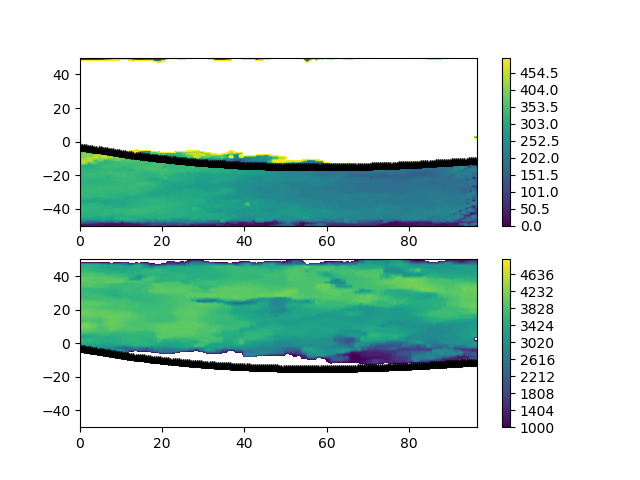
\includegraphics{oppgave_b.png}
	\end{figure}
	\begin{figure}[h!]
		\centering
		\caption{Graf til oppgave \hyperref[ass:c]{c}} 
		\label{fig:c}
		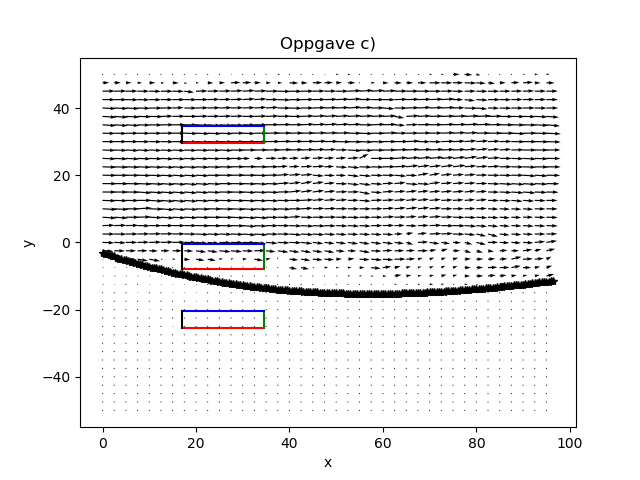
\includegraphics{oppgave_c.png}
	\end{figure}
	\begin{figure}[h!]
		\centering
		\caption{Graf til oppgave \hyperref[ass:d]{d}}
		\label{fig:d}
		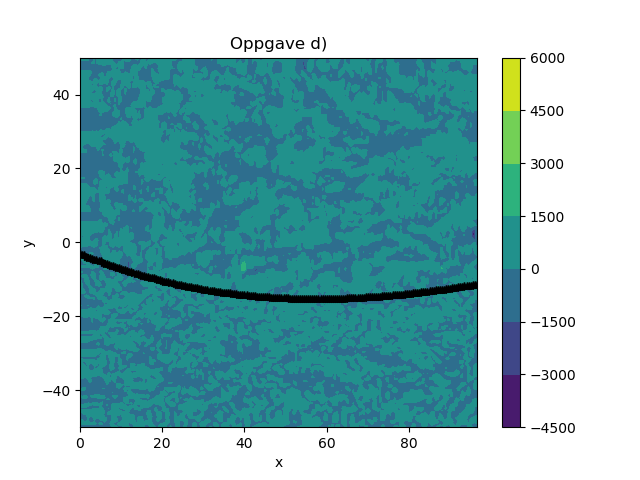
\includegraphics{oppgave_d.png}
	\end{figure}
	\begin{figure}[h!]
		\centering
		\caption{Graf til oppgave \hyperref[ass:e]{e}}
		\label{fig:e}
		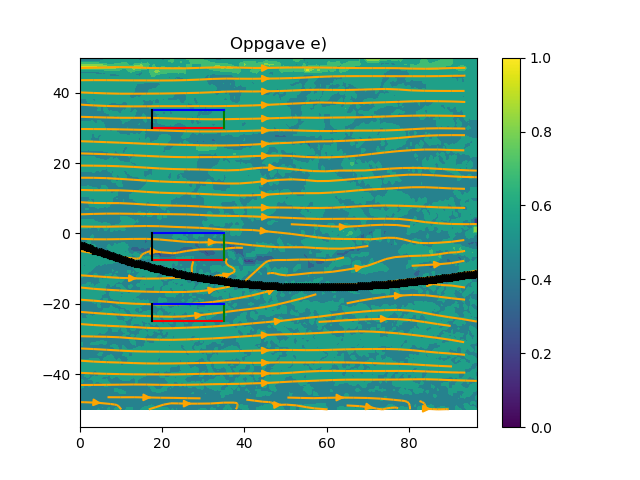
\includegraphics{oppgave_e.png}
	\end{figure}
		
\end{document}
